\documentclass[twoside]{article}

\usepackage{sbc-template}
\usepackage[dvipsnames,usenames,table]{xcolor}
\usepackage{array,booktabs}
\newcounter{tablerow}
\newcommand{\serie}{\parbox{7mm}{\scriptsize\raggedleft\stepcounter{tablerow}\arabic{tablerow}.}~}
\usepackage{graphicx,url}
\graphicspath{{./images/},{../notebooks/CIDDS-2/includes/images}}
\DeclareGraphicsExtensions{.pdf,.png,.jpg}
\usepackage[T1]{fontenc}
\usepackage[utf8]{inputenc}
\usepackage[brazil]{babel}
\usepackage[toc,numberedsection,acronym,translate=babel,acronymlists={hidden}]{glossaries-extra}
\makenoidxglossaries
\setabbreviationstyle[acronym]{short-nolong}
\loadglsentries{./CC-JMG-GLS}
\usepackage{multirow}
\usepackage[multiple]{footmisc}
\renewcommand\thefootnote{\textcolor{red}{\roman{footnote}}}
\usepackage{hyperref}
\usepackage[capitalize,noabbrev,nameinlink,brazilian]{cleveref}
\usepackage[inline]{enumitem}
\usepackage{inconsolata}
\usepackage{calculator}
\usepackage{orcid}
\usepackage{tikz}
\usepackage{forest}
\tikzset{
    darkp/.style={fill=purple!50!black},
    lightp/.style={fill=purple!50}
}
\usepackage{fancyhdr}
\pagestyle{plain}
\usepackage{lastpage}
\rfoot{\thepage \hspace{1pt} - \pageref{LastPage}}

\raggedbottom

\title{Aplicação de Aprendizado de Máquina na Detecção de Intrusão em Redes de Computadores}

\author{
    Carla Cursino\inst{1}\orcidIcon{0000-0002-7718-5897},
    José Marcos Gomes\inst{1}\orcidIcon{0000-0001-9223-7512},
    Ana Carolina Lorena\inst{1}\orcidIcon{0000-0002-6140-571X}, \\
    Filipe Alves Neto Verri\inst{1}\orcidIcon{0000-0002-8240-5129},
    Luiz Alberto Vieira Dias\inst{1}\orcidIcon{0000-0001-5958-8011}
}

\address{Instituto Tecnológico de Aeronáutica - ITA\\
    Divisão da Ciência da Computação - IEC\\
    % Praça Marechal Eduardo Gomes, 50 - Vila das Acácias, 12228-900\\
    São José dos Campos/SP - Brasil    
    \email{cursino@ita.br, gomesjm@ita.br, aclorena@ita.br, verri@ita.br, vdias@ita.br}
}

\begin{document} 

\maketitle

\begin{resumo}\footnotesize
    Sistemas de detecção de intrusão, os chamados \gls{IDS}, trabalham com um sofisticado conjunto de regras e analisam o tráfego de rede em busca de padrões de ataques conhecidos. Os sistemas mais modernos utilizam técnicas de análise de tráfego de redes e procuram analisar o comportamento de usuários e agentes de rede.

    Uma das limitações de tais sistemas é que as regras para detectar intrusão devem ser descritas de antemão para então, analisando o tráfego de rede, o sistema detectar anomalias.
    
    Propomos aplicar métodos de aprendizado de máquina para que o sistema possa antecipar comportamentos anômalos sem a necessidade de existirem regras previamente definidas.
\end{resumo}\normalsize

\section{Introdução}

\glsfmtlong{IDS}. Estes ``sistemas de vigilância e monitoração de ameaças computadorizados'' podem detectar comportamentos ``Suspeitos'' tais como: ``acesso fora do horário usual'', ``frequência de uso além do costumeiro'', ``acesso não usual à dados e programas'', e ``accesso excessivo no volume de dados'' \cite{anderson1980computer}. Dada a importância vital de sistemas computadorizados em nossas vidas, cada vez mais atenção tem sido dada à ferramentas \gls{IDS}, tornando este um componente de grande importância em sistemas de segurança \cite{milenkoski2015evaluating}.

Já as técnicas de invasão se apresentam cada vez mais avançadas, e como consequência os métodos tradicionais baseados em assinaturas ou regras de especialistas não são suficientes \cite{radford2018network} para detectar invasões. Com o passar dos anos, ferramentas \glspl{IDS} baseados em técnicas de aprendizado de máquina tem sido desenvolvidas \cite{milenkoski2015evaluating}.

Pretendemos com este trabalho avaliar abordagens de aprendizado de máquina e determinar o desempenho de sistemas preditivos.

\section{Revisão da Literatura}

Encontramos na literatura abordagens diferentes utilizando aprendizado de máquina aplicada à \glspl{IDS}: o aprendizado supervisionado no qual modelos tentam distinguir entre o tráfego comum do malicioso, e o aprendizado não supervisionado que busca detectar anomalias dentro do tráfego, e o aprendizado semi-supervisionado, onde uma grande quantidade de dados não classificados está disponível juntamento com os dados previamente classificados. 

\subsection{Abordagens Supervisionadas, Semi-supervisionadas e Não Supervisionadas}

O uso de aprendizado supervisionado tem sido amplamente utilizado em sistemas \gls{IDS} \cite{he2017machine} e este método busca classificar o tráfego de rede partindo de um conjunto de dados previamente rotulado de ``Normal'', ``Suspeito'' (e possivelmente ``desconhecido'').

Soluções propostas para resolver o problema de detecção de anomalias por meio da identificação de ``\textit{outliers}'' e ``\textit{inliers}'' podem ser divididas nestas três sub-categorias \cite{aggarwal2016outlier}:

\begin{enumerate}
    \item \textbf{Supervisionadas} - \textit{Lidam com os casos onde o conjunto de dados de treinamento é fornecido com ambos os rótulos (``outliers'' e ``inliers'');}
    \item \textbf{Semi-supervisionada} - \textit{Requer apenas uma classe ``pura'' rotulada ``inlier'' ou ``Normal'';}
    \item \textbf{Não-supervisionada} - \textit{Lida com dados completamente não rotulados e misturados de ``inliers'' e ``outliers''.}
\end{enumerate}

\begin{table}\scriptsize
    \centering
    \begin{tabular}{l l  >{\raggedright\arraybackslash}p{100mm}}
        \toprule
        MÉTODO & ABORDAGEM & DESCRIÇÃO \\
        \midrule
        \textit{Extra Trees} & Supervisionado & Implementa um meta estimador treinado sobre um número de árvores de decisão aleatórias (``\textit{extra trees}'') sobre vários subconjuntos dos dados e calcula a média para melhorar a acurácia de previsão e controlar sobreajustamento. \\
        \textit{KNN} & Supervisionado & Classificador implementando votação em $k$ vizinhos mais próximos. \\
        Bagging & Supervisionado & Um meta-classificador composto que agrupa classificadores de base a subconjuntos aleatórios dos dados originais e agrega as previsões individuais (por votação ou por média) para formar uma previsão final. \\
        \textit{Random Forest} & Supervisionado & Meta classificador que agrupa vários classificadores de árvores de decisão em várias subamostras do conjunto de dados e usa a média para melhorar a precisão e o controle do excesso de ajustes. \\
        \textit{Decision Tree} & Supervisionado & Método que prevê o valor de uma variável alvo, aprendendo regras simples de decisão inferidas a partir das características dos dados. \\
        \textit{Gradient Boosting} & Supervisionado & Constrói um modelo aditivo de modo progressivo que permite a otimização de funções de perda diferenciadas arbitrárias. \\
        \textit{Ada Boost} & Supervisionado & Meta-classificador que se inicia com um classificador no conjunto de dados original e depois adiciona cópias do classificador sobre o mesmo conjunto de dados, onde os pesos das instâncias classificadas incorretamente são ajustados de tal forma que os classificadores subsequentes se concentram mais nos casos difíceis. \\
        \textit{One Class SVM} & Não-supervisionado & Detector de pontos fora da curva não supervisionado que implementa Máquina de Suporte à Vetores. \\
        \bottomrule
    \end{tabular}
    \caption{Métodos abordados neste estudo}
    \label{tab:metodos}
\normalsize\end{table}

Para este estudo previlegiamos algoritmos computacionalmente menos exigentes e que viabilizariam a implementação de  análise em tempo real de eventos de rede.

\subsection{Modelos}

\subsubsection{Lineares}

Para funcionarem adequadamente num modelo linear, os dados precisam ser altamente correlacionados e quando os dados não o forem e altamente agrupados em certas regiões este método é ineficaz. Estudos sugerem que correlações podem ser específicas para determinadas localidades de dados e neste caso subespaços globais localizados por \gls{PCA} por exemplo são subótimas para detecção de \textit{outliers} \cite{aggarwal2000finding}.

\subsubsection{Baseados em Proximidade}

Num problema multidimensional como o de detecção de anomalias em eventos de redes de computadores os pontos acabam por se mostrarem equidistantes um do outro e assim o contraste de diferenças é perdido \cite{aggarwal2001surprising,hinneburg2000nearest}.

\subsubsection{Probabilísticos}

Modelos paramétricos são muito suscetíveis à ruidos e sobreajustes. A escolha incorreta de parâmetros pode levar à classificação de dados espúrios como \textit{outliers} ou quando o modelo é muito genérico o número de parâmetros necessários para descrevê-lo se torna proibitivo fazendo com que \textit{outliers} se percam em resultado de sobreajuste e na redução do sobreajuste para resolver o problema acabamos incorrendo em subajuste.

\section{Materiais e Métodos}

\subsection{Conjunto de Dados}

Para este trabalho utilizamos o conjunto de dados \textbf{CIDDS-001} (``\textit{Coburg Intrusion Detection Data Sets}''), cujo conceito é o de criar um conjunto de dados para avaliação de sistemas de detecção de intrusão \cite{ring2017creation,ring2017flow}.

O conjunto de dados é composto por dois grupos de arquivos, um de acessos de origem externa e outro de origem interna. Cada grupo está segmentado em arquivos de captura de dados contendo uma semana de observações, num total de oito arquivos no formato \textbf{CSV}.

Dado o grande número de dados, trabalhamos com uma amostragem dos dados totais.

\begin{table}\scriptsize
    \centering
    \begin{tabular}{rl}
        \toprule
        AMOSTRAS &  ARQUIVO \\
        \midrule
           172.838 & CIDDS-001-external-week1.csv \\
           159.374 & CIDDS-001-external-week2.csv \\
           153.027 & CIDDS-001-external-week3.csv \\
           186.005 & CIDDS-001-external-week4.csv \\
         8.451.521 & CIDDS-001-internal-week1.csv \\
        10.310.734 & CIDDS-001-internal-week2.csv \\
         6.349.784 & CIDDS-001-internal-week3.csv \\
         6.175.898 & CIDDS-001-internal-week4.csv \\
        31.959.181 & TOTAL \\
        \bottomrule
    \end{tabular}
    \caption{Conjuntos de dados CIDDS}
    \label{tab:tab:dataset}
\normalsize\end{table}

\begin{itemize}
    \item \texttt{Date first seen~~ - object } - Data e hora do início da sessão
    \item \texttt{Duration~~~~~~~~~ - float64} - Duração da sessão (em milisegundos)
    \item \texttt{Proto~~~~~~~~~~~~ - object } - Protocolo
    \item \texttt{Src IP Addr~~~~~~ - object } - \glsfmtshort{IP} de origem
    \item \texttt{Src Pt~~~~~~~~~~~ - int64~~} - Porta de origem
    \item \texttt{Dst IP Addr~~~~~~ - object } - \glsfmtshort{IP} de destino
    \item \texttt{Dst Pt~~~~~~~~~~~ - float64} - Porta de destino
    \item \texttt{Packets~~~~~~~~~~ - int64~~} - Número de pacotes
    \item \texttt{Bytes~~~~~~~~~~~~ - object } - Número de \glspl{byte}
    \item \texttt{Flows~~~~~~~~~~~~ - int64~~} - Quantidade de fluxos de transmissão
    \item \texttt{Flags~~~~~~~~~~~~ - object } - Indicadores \glsfmtshort{TCP}
    \item \texttt{ToS~~~~~~~~~~~~~~ - int64~~} - Tipo de serviço
    \item \texttt{class~~~~~~~~~~~~ - object } - Classificação do ataque
    \item \texttt{attackType~~~~~~~ - object } - Tipo de ataque
    \item \texttt{attackID~~~~~~~~~ - object } - Identificação do ataque
    \item \texttt{attackDescription - object } - Descrição do ataque
\end{itemize}

\subsection{Técnicas}

Para tratar a natureza desbalanceada dos dados classificados (ver \cref{fig:umbalanced-class}), foi aplicado tanto ``\textit{Upsample}'' da classe minoritária quanto ``\textit{Downsample}'' da classe majoritária e os desempenhos dos métodos de classificação foram comparados.

\begin{figure}
    \centering
    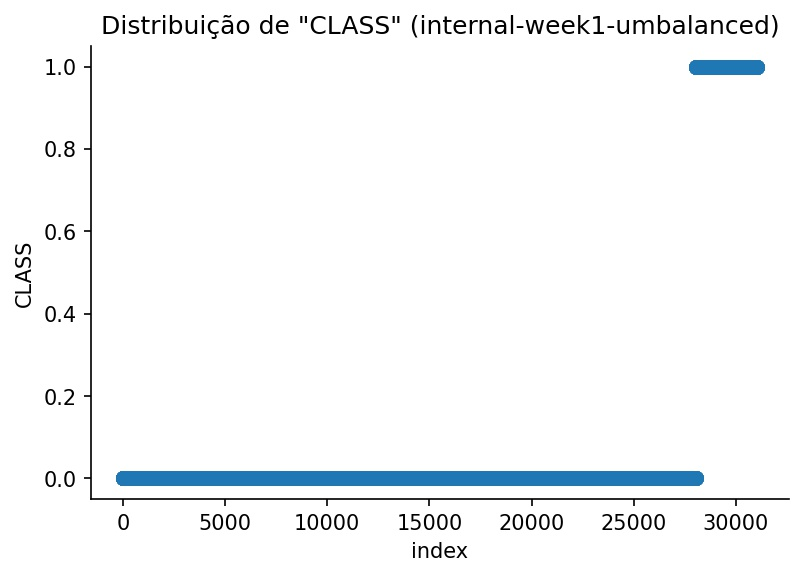
\includegraphics[width=0.45\textwidth]{distribuicao-internal-week1-umbalanced-CLASS.jpg}
    \caption{Distribuição da classe}\label{fig:umbalanced-class}
\end{figure}

\section{Experimentos e Resultados}

Curva ``\textit{Receiver Operating Characteristic}'' (\textbf{ROC}) é uma ferramenta importante de diagnóstico do desempenho de algoritmos de aprendizado de máquina que nos mostra a taxa de verdadeiros positivos contra falsos negativos. A área sob a curva \textbf{ROC} é chamada de \textbf{AUC} é uma medida de previsibilidade do algorítmo. Um \textbf{AUC} mais alto indica uma previsão mais apurada.

\subsection{Exploração de Dados}

\subsubsection{Atributos Mais Significativos}

\begin{enumerate}
    \setcounter{enumi}{2}
    \item \textit{Proto} - Protocolos de comunicação
    \setcounter{enumi}{10}
    \item \textit{Flags} - Indicadores \glsfmtshort{TCP} - cada \gls{bit} dos $16$ (apenas $8$ estão em uso) são reservados para este atributo e identificados como: 
        \begin{itemize}
            \item \textbf{CWR} - \gls{bit} $7$ - ``\textit{Congestion Window Reduction}'' - identificado pela letra \textbf{C}
            \item \textbf{ECE} - \gls{bit} $6$ - ``\textit{ECN (Explicit Congestion Notification) Capable}'' - identificado pela letra \textbf{E}
            \item \textbf{URG} - \gls{bit} $5$ - ``\textit{Urgent}'' - identificado pela letra \textbf{U}
            \item \textbf{ACK} - \gls{bit} $4$ - ``\textit{Acknowledgement}'' - identificado pela letra \textbf{A}
            \item \textbf{PSH} - \gls{bit} $3$ - ``\textit{Push}'' - identificado pela letra \textbf{P}
            \item \textbf{RST} - \gls{bit} $2$ - ``\textit{Reset}'' - identificado pela letra \textbf{R}
            \item \textbf{SYN} - \gls{bit} $1$ - ``\textit{Synchronization}'' - identificado pela letra \textbf{S}
            \item \textbf{FIN} - \gls{bit} $0$ - ``\textit{Finished}'' - identificado pela letra \textbf{F}
        \end{itemize}
        Valores que estão fora do padrão determinados pela \gls{IETF} e documentados pelo \gls{IEEE} no conjunto de dados deverão ser traduzidos:
        \begin{itemize}
            \item \texttt{0xDB} - \texttt{11011011} - \texttt{CE.AP.SF}
            \item \texttt{0xD2} - \texttt{11010010} - \texttt{CE.A..S.}
            \item \texttt{0xC2} - \texttt{11000010} - \texttt{CE....S.}
            \item \texttt{0xDA} - \texttt{11011010} - \texttt{CE.AP.S.}
            \item \texttt{0xD7} - \texttt{11010111} - \texttt{CE.A.RSF}
            \item \texttt{0x53} - \texttt{01010011} - \texttt{.E.A..SF}
            \item \texttt{0xDF} - \texttt{11011111} - \texttt{CE.APRSF}
            \item \texttt{0xD6} - \texttt{11010110} - \texttt{CE.A.RS.}
            \item \texttt{0xD3} - \texttt{11010011} - \texttt{CE.A..SF}
        \end{itemize}
        \setcounter{enumi}{12}
    \item \textit{class} - Classificação (atributo alvo)
\end{enumerate}

Os protocolos \gls{ICMP} \cite{postel1981ietf} e \gls{GRE} \cite{farinacci2000rfc2784} não são geralmente iniciados ou recebidos em comunicações normais e podem ser aplicados por vetores de ataque e não podem ser negligenciados. Já os protocolos \gls{TCP} \cite{postel1981transmission} e \gls{UDP} \cite{protocol1980rfc} representam toda a comunicação via Internet com que os usuários costumam interagir normalmente. Endereços e portas \gls{IP} também serão desconsiderados, mesmo porque atacantes costumam mascarar seus endereços e o uso de \gls{NAT} pela maioria das redes para publicar serviços externos limita a utilidade de analisar esta informação \cite{deabordagem}.

\begin{table}\scriptsize
    \centering
    \begin{tabular}{lrlrlll}
\toprule
{} &      DURATION & PROTOCOL &       PACKETS &     BYTES &    FLAGS &    CLASS \\
\midrule
count  &  8.451520e+06 &  8451520 &  8.451520e+06 &   8451520 &  8451520 &  8451520 \\
unique &  0.000000e+00 &        4 &  0.000000e+00 &     89693 &       20 &        3 \\
top    &  0.000000e+00 &    TCP   &  0.000000e+00 &        66 &   .A.... &   normal \\
freq   &  0.000000e+00 &  7393818 &  0.000000e+00 &   2279907 &  2652182 &  7010897 \\
mean   &  1.141597e-01 &        0 &  1.503053e+01 &         0 &        0 &        0 \\
std    &  7.683694e-01 &        0 &  9.768317e+02 &         0 &        0 &        0 \\
min    &  0.000000e+00 &        0 &  1.000000e+00 &         0 &        0 &        0 \\
25\%    &  0.000000e+00 &        0 &  1.000000e+00 &         0 &        0 &        0 \\
50\%    &  0.000000e+00 &        0 &  2.000000e+00 &         0 &        0 &        0 \\
75\%    &  2.500000e-02 &        0 &  4.000000e+00 &         0 &        0 &        0 \\
max    &  2.244120e+02 &        0 &  2.087680e+05 &         0 &        0 &        0 \\
\bottomrule
\end{tabular}

    \caption{Estatísticas dos dados brutos}
    \label{tab:val_stat_before_pre}
\normalsize\end{table}  

\subsubsection{Análise de Dispersão e Distribuição}

\begin{table}\scriptsize
    \centering
    \begin{tabular}{lr}
\toprule
 FEATURE &     KURTOSIS \\
\midrule
DURATION &  3035.547966 \\
PROTOCOL &     2.521929 \\
 PACKETS & 13423.894329 \\
   BYTES & 25936.752752 \\
   FLAGS &    -1.380831 \\
   CLASS &     5.502495 \\
\bottomrule
\end{tabular}

    \caption{Curtose}
    \label{tab:kurt}
\normalsize\end{table}  

\begin{table}\scriptsize
    \centering
    \begin{tabular}{lr}
\toprule
 FEATURE &       SKEW \\
\midrule
DURATION &  47.795086 \\
PROTOCOL &   2.041001 \\
 PACKETS & 111.699528 \\
   BYTES & 157.458199 \\
   FLAGS &   0.235055 \\
   CLASS &   2.739003 \\
\bottomrule
\end{tabular}

    \caption{Obliquidade}
    \label{tab:skew}
\normalsize\end{table}  

\begin{table}\scriptsize
    \centering
    \begin{tabular}{rrrrrr}
\toprule
 DURATION &  PROTOCOL &  PACKETS &  BYTES &  FLAGS &  CLASS \\
\midrule
        0 &         1 &        1 &     66 &      4 &      0 \\
\bottomrule
\end{tabular}

    \caption{Moda}
    \label{tab:mode}
\normalsize\end{table}  

Comparando a curtose (ver \cref{tab:kurt}) com a média e a mediana (ver \cref{tab:umbalanced_stat_after_pre}), observamos aquela bem acima destas e um grande número de objetos ocorrem frequentemente fora da distribuição ``Normal''. A obliquidade de todos estes atributos é positiva (ver \cref{tab:skew}), e a maioria dos valores tendem ao mínimo e está associada ao grande desvio padrão observado nos atributos ``\textit{Duration}'' e ``\textit{Bytes}''.

\subsection{Pré-processamento}

Tratamos os dados de forma uniforme para todos os algoritmos testados e geramos três conjuntos de dados:

\begin{enumerate}
    \item Não balanceado - onde foram preservados os dados originais e aplicadas apenas normalização de valores;
    \item \textit{Upsample} - onde aplicamos \textit{Upsampling} da classe minoritária; e
    \item \textit{Downsample} - onde aplicamos \textit{Downsampling} da classe majoritária.
\end{enumerate}

\begin{table}\scriptsize
    \centering
    \begin{tabular}{lrrrrrr}
\toprule
{} &      DURATION &      PROTOCOL &       PACKETS &         BYTES &         FLAGS &         CLASS \\
\midrule
count &  31029.000000 &  31029.000000 &  31029.000000 &  3.102900e+04 &  31029.000000 &  31029.000000 \\
mean  &      0.001224 &      0.567550 &      0.000102 &  5.501999e-05 &      0.380647 &      0.096200 \\
std   &      0.013110 &      0.172793 &      0.007367 &  5.950411e-03 &      0.269249 &      0.294871 \\
min   &      0.000000 &      0.000000 &      0.000000 &  0.000000e+00 &      0.000000 &      0.000000 \\
25\%   &      0.000000 &      0.500000 &      0.000000 &  6.934413e-08 &      0.222222 &      0.000000 \\
50\%   &      0.000000 &      0.500000 &      0.000006 &  2.600405e-07 &      0.222222 &      0.000000 \\
75\%   &      0.000000 &      0.500000 &      0.000018 &  1.262641e-06 &      0.666667 &      0.000000 \\
max   &      1.000000 &      1.000000 &      1.000000 &  1.000000e+00 &      1.000000 &      1.000000 \\
\bottomrule
\end{tabular}

    \caption{Estatísticas após o pré-processamento (dados originais)}
    \label{tab:umbalanced_stat_after_pre}
\normalsize\end{table}  

\subsection{Experimentos}

Nas \cref{tab:superv-umbalanced,tab:superv-upsample,tab:superv-downsample} comparamos os resultados dos experimentos.

\begin{table}\scriptsize
    \centering
    \begin{tabular}{lrrr}
\toprule
        Algoritmo &  Acurácia &  Precisão &      AUC \\
\midrule
              KNN &  0.999355 &  0.995871 & 0.996528 \\
      Extra Trees &  0.998550 &  0.995510 & 0.996084 \\
    Random Forest &  0.997261 &  0.994932 & 0.995373 \\
          Bagging &  0.997100 &  0.994860 & 0.995284 \\
   Decistion Tree &  0.996777 &  0.994716 & 0.995107 \\
Gradient Boosting &  0.992749 &  0.992579 & 0.992887 \\
        Ada Boost &  0.986465 &  0.983349 & 0.983968 \\
\bottomrule
\end{tabular}

    \caption{Semana 1 - não balanceado}
    \label{tab:superv-umbalanced}
\normalsize\end{table}  

\begin{table}\scriptsize
    \centering
    \begin{tabular}{lrrr}
\toprule
        Algoritmo &  Acurácia &  Precisão &      AUC \\
\midrule
      Extra Trees &  0.995812 &  0.991809 & 0.996013 \\
Gradient Boosting &  0.995812 &  0.991809 & 0.996013 \\
    Random Forest &  0.995812 &  0.991809 & 0.996013 \\
              KNN &  0.995812 &  0.991809 & 0.996013 \\
          Bagging &  0.994975 &  0.991854 & 0.995131 \\
   Decistion Tree &  0.994975 &  0.991854 & 0.995131 \\
        Ada Boost &  0.993300 &  0.992960 & 0.993283 \\
\bottomrule
\end{tabular}

    \caption{Semana 1 - ``\textit{Upsampling}''}
    \label{tab:superv-upsample}
\normalsize\end{table}  

\begin{table}\scriptsize
    \centering
    \begin{tabular}{lrrr}
\toprule
        Algoritmo &  Acurácia &  Precisão &      AUC \\
\midrule
      Extra Trees &  0.997504 &  0.997149 & 0.997504 \\
              KNN &  0.997237 &  0.996965 & 0.997236 \\
          Bagging &  0.996613 &  0.996072 & 0.996612 \\
    Random Forest &  0.996523 &  0.995894 & 0.996523 \\
   Decistion Tree &  0.995097 &  0.993032 & 0.995095 \\
Gradient Boosting &  0.991442 &  0.987837 & 0.991439 \\
        Ada Boost &  0.984667 &  0.980849 & 0.984663 \\
\bottomrule
\end{tabular}

    \caption{Semana 1 - ``\textit{Downsampling}''}
    \label{tab:superv-downsample}
\normalsize\end{table}

\begin{table}\scriptsize
    \centering
    \begin{tabular}{lrrrrrrr}
\toprule
               Algoritmo &  Acurácia &  Precisão &      AUC &  F1 (Normal) &  F1 (Suspeito) &  MCC (Normal) &  MCC (Suspeito) \\
\midrule
  One Class SVM (Linear) &  0.917499 &  0.217552 & 0.584388 &     0.956232 &       0.282913 &      0.332133 &        0.332133 \\
One Class SVM (Sigmoid) &  0.917499 &  0.217552 & 0.584388 &     0.956232 &       0.282913 &      0.332133 &        0.332133 \\
     One Class SVM (RBF) &  0.805833 &  0.648940 & 0.714537 &     0.885380 &       0.365456 &      0.304000 &        0.304000 \\
\bottomrule
\end{tabular}

    \caption{Semana 1 - não supervisionado}
    \label{tab:nao-superv-umbalanced}
\normalsize\end{table}

Aplicamos sobre os conjunto de dados os algoritmos (ver \cref{tab:metodos}), divididos em dois grupos, os \textbf{Supervisionados} (onde selecionamos 7 algoritmos, sendo cinco \textit{Ensembles}, 1 de \textit{Árvore} de decisão, e 1 de \textit{Proximidade}) e um \textbf{Não supervisionado} dentro do subgrupo de \textit{Support Vector Machine}. O principal fator de escolha dos algoritmos é o de baixo custo computacional, e assim sendo, desprezamos Redes Neurais e outros que podem vir a ser computacionalmente intensos.

\section{Discussão}

Os resultados obtidos e listados nas \cref{tab:superv-umbalanced,tab:superv-upsample,tab:superv-downsample} mostram uma ``\textit{acurácia}'' ($ACC$) bastante próxima em todos os modelos experimentados (entre $98.6\%$ com \textbf{Ada Boost} a até $99.9\%$ com \textbf{KNN}, todos aplicados sobre dados não balanceados). 
    
Comparando os algoritmos entre si, \textbf{Extra Trees} se destacou aplicada à dados balanceados com \textit{Upsampling} e \textit{Downsampling} ou não balanceados, com acurácia de $99.5\%$, $99.7\%$ e $99.8\%$ respectivamente. Curiosamente \textbf{Gradient Boosting} destacou-se aplicando-se \textit{Upsampling} aos dados, com $99.5\%$, porém ficou ligeiramente aquém das demais aos aplicarmos \textit{Downsampling}, com $99.1\%$.

No geral todos os algoritmos se mostraram consistentes e indiferentes ao tratamento às classes das observações da amostra de dados e o impacto da distribuição de classes não foi significativo sobre os algoritmos experimentados. Creditamos isto à natureza do conjunto de dados que não possui um espectro muito variado de ataques disponíveis (para gerar o tráfego malicioso são simulados ataques do tipo \textit{Denial of Service (DoS)}, ataques de força bruta e escrutíno de portas \cite{ring2017creation,ring2017flow}).

Comparando o desempenho com o algoritmo não supervisionado \textbf{One Class SVM} aplicado aos dados não balanceados, que pode ser observado na \cref{tab:nao-superv-umbalanced}, atingiu acurácia de $80.5\%$ (a mais baixa) a até $91.7\%$ com diferentes \textit{kernels} (tanto ``\textbf{Linear}'' quanto ``\textbf{Sigmoid}'' apresentaram o mesmo desempenho, enquanto que ``\textbf{RBF}'' foi inferior), onde $\nu = 0.125$ para todos os casos.

A pontuação $F_1$ é outra medida de verificação da ``\textit{acurácia}'' de um modelo, dada pela média harmônica entre a precisão e \textit{recall}:

\begin{align*}
    F_1 = \frac{TP}{TP + \frac{1}{2}(FP + FN)} \text{,}
\end{align*}

\noindent onde:

\begin{itemize}
    \item $TP$: \textit{True Positive} - Verdadeiro Positivo;
    \item $FP$: \textit{False Positive} - Falso Positivo; e
    \item $FN$: \textit{False Negative} - Falso Negativo.
\end{itemize}

A pontuação $F_1$ de observações classificadas como ``\textbf{Suspeitas}'' é significativamente inferior ($36.5\%$ usando ``\textbf{RBF}'' e $28.2\%$ para os demais ``\textit{kernels}'') à das classificadas como ``\textbf{Normais}'' ($88.5\%$ ``\textbf{RBF}'' e $95.6\%$ para os demais ``\textit{kernels}''), o que indica uma tendência do modelo a identificar como ``Suspeitos'' eventos de classe ``Normal''.

Aplicamos o coeficiente de correlação \textit{Matthews} como uma medida da qualidade da classificação binária de nosso modelo. Esta medida leva em consideração verdadeiros e falsos positivos e negativos e é considerada uma medida balanceada em classes desbalanceadas, que retorna valores entre $+1$ (uma previsão perfeita) e $-1$ (discordância total entre observação e previsão), enquanto que $0$ indica que a previsão é tão boa quanto uma previsão aleatória \cite{matthews1975comparison}:

\begin{align*}
    | MCC | = \sqrt{\frac{x^2}{n}} \text{,}
\end{align*}

\noindent onde $n$ é número total de observações, ou a partir da matriz de confusão:

\begin{align*}
    MCC = \frac{TP \times TN - FP \times FN}{\sqrt{(TP + FP) \times (TP + FN) \times (TN + FP) \times (TN + FN)}} \text{,}
\end{align*}

\noindent onde:

\begin{itemize}
    \item $TP$: \textit{True Positive} - Verdadeiro Positivo;
    \item $TN$: \textit{True Negative} - Verdadeiro Negativo;
    \item $FP$: \textit{False Positive} - Falso Positivo; e
    \item $FN$: \textit{False Negative} - Falso Negativo.
\end{itemize}

A pontuação $MCC$ nos dá o ``\textbf{produto - momento}'' do coeficiente de correlação \textit{Pearson} (diferente do próprio coeficiente de correlação \textit{Pearson} que mede a relação entre os coeficientes), que com o valor $30.4\%$ (para ambas as classes) usando ``\textit{kernel}'' ``\textbf{RBF}'' e $33.2\%$ para os demais é interpretado como uma previsão ``\textbf{Fraca}'' e próxima de ``\textit{Negligenciável}'' (ver \cref{tab:mcc}) \cite{powers2020evaluation}.

\begin{table}\scriptsize
    \centering
    \begin{tabular}{rl}
        \toprule
            MCC &  Interpretação \\
        \midrule
        $[0.0, 0.3)$ & \textit{Negligenciável} \\
        $[0.3, 0.5)$ & \textit{Fraca} \\
        $[0.5, 0.7)$ & \textit{Moderada} \\
        $[0.7, 0.9)$ & \textit{Forte} \\
        $[0.9, 1.0]$ & \textit{Muito Forte} \\
        \bottomrule
        \end{tabular}
    \caption{Interpretação do coeficiente de correlação \textit{Matthews}}
    \label{tab:mcc}
\normalsize\end{table}

\section{Conclusões e trabalhos futuros}

Apresentamos uma análise de modelos de aprendizado aplicado ao conjunto de dados de estudos em intrusão de redes \textbf{CIDDS}. Obtivemos sucesso na identificação de eventos de invasão com uma acurácia de $99\%$ utilizando modelos supervisionados. 

As diferenças entre os conjuntos de dados tratados ou não com \textit{Upsampling} e \textit{Downsampling} não foram significativas o suficiente para justificarem este tratamento que pode ser custoso para este caso particular e uma análise detalhada de conjuntos de dados não balanceados deveria ser aplicada antes \cite{barella2021assessing}.

Comparamos com um modelo de detecção não supervisionado que apresentou uma acurácia de $80\%$, porém como podemos observar após uma análise mais detalhada utilizando o coeficiente de correlaçao \textit{Matthews}, atingiu uma pontuação entre $30\%$ e $33\%$, considerado um fator de previsão ``\textbf{Fraco}''. 

Modelos de detecção utilizando algoritmos não supervisionados podem vir a ser explorado com o intuito de obtermos índices de acurácia próximos dos modelos preditivos supervisionados, e com fatores de previsão melhores que os apresentados pelo algoritmo \textbf{One Class SVM} neste exercício.

\footnotesize{
    \printnoidxglossary[type=acronym]
    \printnoidxglossary[type=main]
}\normalsize

\section{Referências}

    \bibliographystyle{acm}
    \begingroup
        \renewcommand{\section}[2]{}
        \footnotesize{
            \bibliography{CC-JMG}
        }\normalsize
    \endgroup

\end{document}